\chapter{Árboles parcialmente ordenados}
Un \textbf{árbol parcialmente ordenado} o \textbf{APO}, es un árbol completo (árbol que tiene todos sus niveles llenos menos el último que faltan nodos por la derecha) en el que el \textit{valor de cualquier nodo es menor o igual que el de todos sus descendientes}. 
\begin{figure}[h]
  \begin{center}
    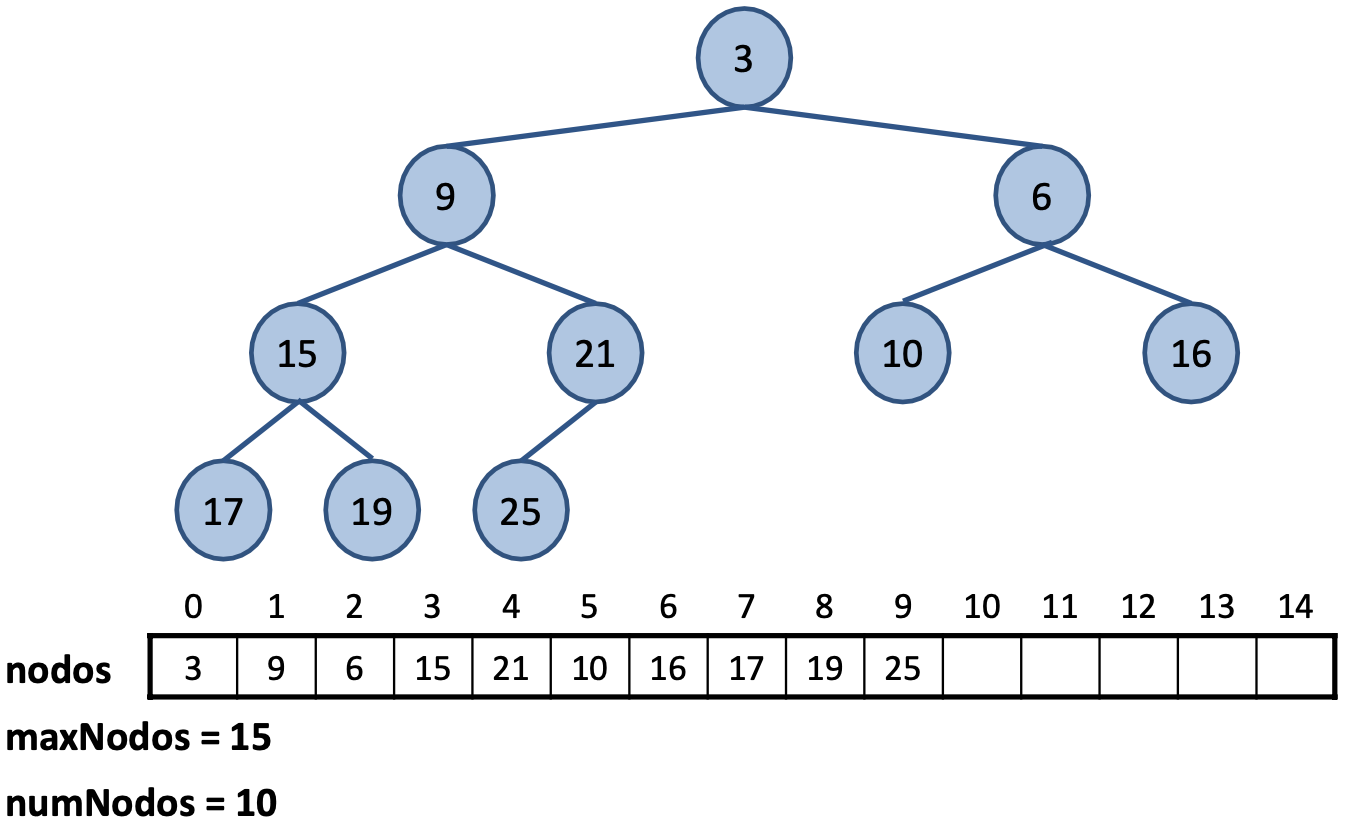
\includegraphics[width=0.7\textwidth]{assets/apo1.png}
  \end{center}
\end{figure}
\section{Operaciones básicas}
Cuando trabajamos con APOs podemos realizar varias operaciones como \textbf{acceso al mínimo valor}, \textbf{inserción} y \textbf{eliminación}.
\begin{itemize}
  \item El mínimo valor se puede obtener en un tiempo de\(O(1)\), debido a que el mínimo valor siempre será la \textbf{raíz} del propio árbol.
  \item Encontramos la \textbf{propiedad de completitud} que implica que la altura menor posible del APO de \(n\) nodos es de \(h = log_{2}\ n\).
  \item También existe la \textbf{propiedad de orden} del APO que permite efectuar inserciones y eliminaciones en el mismo en un tiempo \(O(h)\) (en el peor caso), y en un tiempo \(O(log_{2}\ n)\) en el mejor y caso promedio.
\end{itemize}

\section{Especificación del TAD árbol parcialmente ordenado}
En los árboles parcialmente ordenados vamos a encontrar dos métodos \texttt{hundir()} y \texttt{flotar()}.

\subsection*{Constructor del árbol parcialmente ordenado}
\underbar{\textit{Precondición:}} maxNodos $>$ 0\\
\underbar{\textit{Postcondición:}} Crea y devuelve un APO de tamaño MaxNodos vacío.\\
\verb|  Apo(size_t maxNodos);|

\subsection*{Inserción de elementos en el APO}
\underbar{\textit{Precondición:}} APO no lleno.\\
\underbar{\textit{Postcondición:}} Inserta el elemento en su posición correcta.\\
\verb|  void insertar(const T& e);|
\subsection*{Eliminación de elementos en el APO}
\underbar{\textit{Precondición:}} APO no vacío.\\
\underbar{\textit{Postcondición:}} Elimina la raíz reordenando el APO.
\verb|  void suprimir();|
\subsection*{Métodos observadores de un APO}
\begin{itemize}
  \item \underbar{\large\textbf{Obtener la raíz}}:\\
  \underbar{\textit{Precondición:}} APO no vacío.\\
  \underbar{\textit{Postcondición:}} Devuelve el elemento que está en la raíz.\\
  \verb|  const T& cima()const;|
  \item \underbar{\large\textbf{Obtener estado del árbol}}:\\
  \underbar{\textit{Postcondición:}} Devuelve \texttt{True} si el árbol está vacío, si no, \texttt{False}.
  \verb|  bool vacio()const;|
  \item \underbar{\large\textbf{Obtener el padre}}:\\
  \underbar{\textit{Precondición:}} APO no vacío.\\
  \underbar{\textit{Postcondición:}} Devuelve el padre del nodo n.\\
  \verb|nodo padre(nodo n)const;|
  \item \underbar{\large\textbf{Obtener el hijo izquierdo}}:\\
  \underbar{\textit{Precondición:}} APO no vacío.\\
  \underbar{\textit{Postcondición:}} Devuelve el hijo izquierdo del nodo \(n\).\\
  \verb|nodo hIzq(nodo n)const;|
  \item \underbar{\large\textbf{Obtener el hijo derecho}}:\\
  \underbar{\textit{Precondición:}} APO no vacío.\\
  \underbar{\textit{Postcondición:}} Devuelve el hijo derecho del nodo \(n\).\\
  \verb|  nodo hDer(nodo n)const;|
\end{itemize}


\subsection*{Métodos hundir y flotar de un APO}
\begin{itemize}
  \item \underbar{\large\textbf{Hundir un nodo}}:\\
  Este método irá de la mano a la hora de eliminar el nodo raíz, reordenando el árbol hasta que dicho nodo sea una hoja y lo podamos eliminar.

  Podemos tener 3 casos a la hora de eliminar la raíz del APO:
  \begin{itemize}
    \item \textbf{Caso 1: Un nodo} → Al tener un solo nodo (raíz), si la eliminamos el árbol quedará \textbf{vacío}.
    \item \textbf{Caso 2: Dos nodo} → Ahora tenemos tanto la raíz como su hijo izquierdo, por tanto, si eliminamos la raíz, su hijo izquierdo pasará a ser la nueva raíz del APO.
    \item \textbf{Caso 3: Más de dos nodo} → Si queremos eliminar una raíz que tiene más de dos nodos, el último nodo insertado será el que ocupe la posición del raíz y luego hundimos dicho nodo para poder cumplir la propiedad de orden.
  \end{itemize}
  \verb|  void hundir(nodo n);|
  \item \underbar{\large\textbf{Flotar un nodo}}:\\
  A la hora de insertar un nodo, éste se añade a la última posición del vector y luego para que se cumpla la propiedad de orden tenemos que ir `subiendo' dicho nodo hasta que encuentre su sitio.

  \verb|  void flotar(nodo n);|
\end{itemize}
\section{Implementación del TAD árbol parcialmente ordenado}
Vamos a hacer uso de la implementación mediante un \textbf{vector de posiciones relativas} ya que estos son muy útiles y eficientes cuando trabajamos con árboles completos.

La parte privada del TAD quedaría:
\begin{minted}[breaklines]{C++}
template <typename T> class Apo{
  public:
    //Métodos vistos en la Especificación del TAD.
  private:
    typedef size_t nodo; //Indice del vector.
    size_t maxNodos; //Tamaño del vector (árbol).
    size_t numNodos; //Número de nodos (último nodo del árbol)
    T* nodos; //Vector de nodos
    //Métodos privados de la clase
    nodo padre(nodo n)const;
    nodo hIzq(nodo n)const;
    nodo hDer(nodo n)const;
    void hundir(nodo n);
    void floar(nodo n);
};
\end{minted}
\newpage
\subsection*{Inserción de elementos en un APO}
\begin{figure}[h]
  \begin{center}
    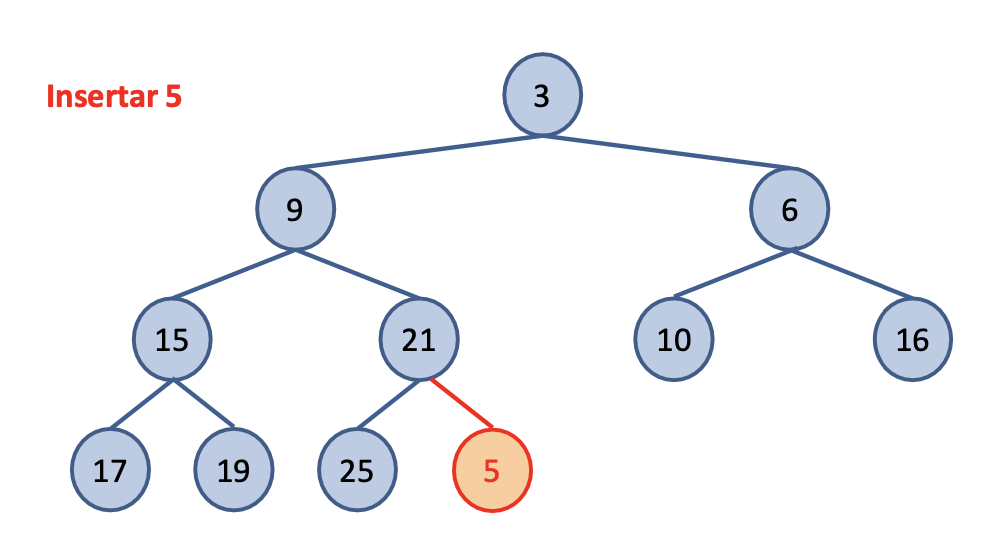
\includegraphics[width=0.7\textwidth]{assets/apo2.png}
  \end{center}
  \caption{Ejemplo de inserción 1.}
\end{figure}
Queremos insertar el valor `5' en nuestro APO el cual no está vacío, por tanto, vamos a insertarlo en la última posición del vector de posiciones relativas que equivale al hijo derecho del nodo con valor `21'. A continuación vamos flotando dicho nodo hasta que se cumpla la propiedad de ordenación.
\begin{figure}[h]
  \begin{center}
    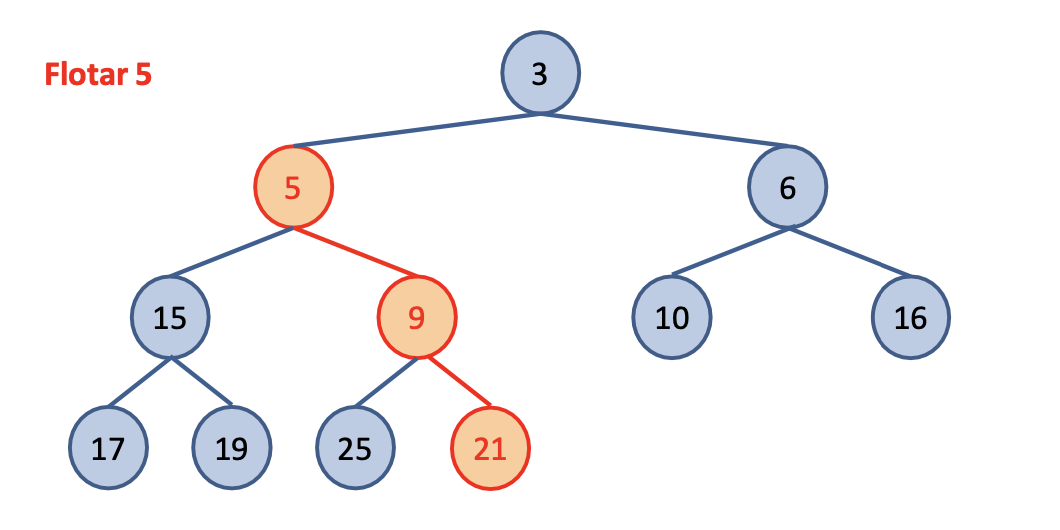
\includegraphics[width=0.7\textwidth]{assets/apo3.png}
  \end{center}
  \caption{Ejemplo de inserción 2.}
\end{figure}
Tenemos como resultado que el nodo con valor `5' es el nuevo hijo izquierdo del nodo raíz, y por tanto, vemos que todos los nodos están ordenados.
\subsubsection*{Código de Inserción y Flotar}

\underbar{Código de insertar:}
\begin{minted}[breaklines]{C++}
template <typename T> void Apo<T>::insertar(const T& e){
  assert(numNodos < maxNodos);
  //insertamos en la última posición.
  nodos[numNodos] = e; 
  //Llamamos al método flotar
  if(numNodos > 1)
    flotar(numNodos-1);
}
  \end{minted}
\underbar{Código de flotar:}
\begin{minted}[breaklines]{C++}
template <typename T> void Apo<T>::flotar(nodo n){
  //Guardamos el contenido del nodo
  T e = nodos[n];
  //recorremos los nodos intercambiandolos
  while(n>0 && e < nodos[padre(n)]){
    nodos[n] = nodos[padre(n)];
    n = padre(n);
  }
  nodos[n] = e;
}
\end{minted}

\subsection*{Eliminación de elementos en un APO}
\begin{figure}[h]
  \begin{center}
    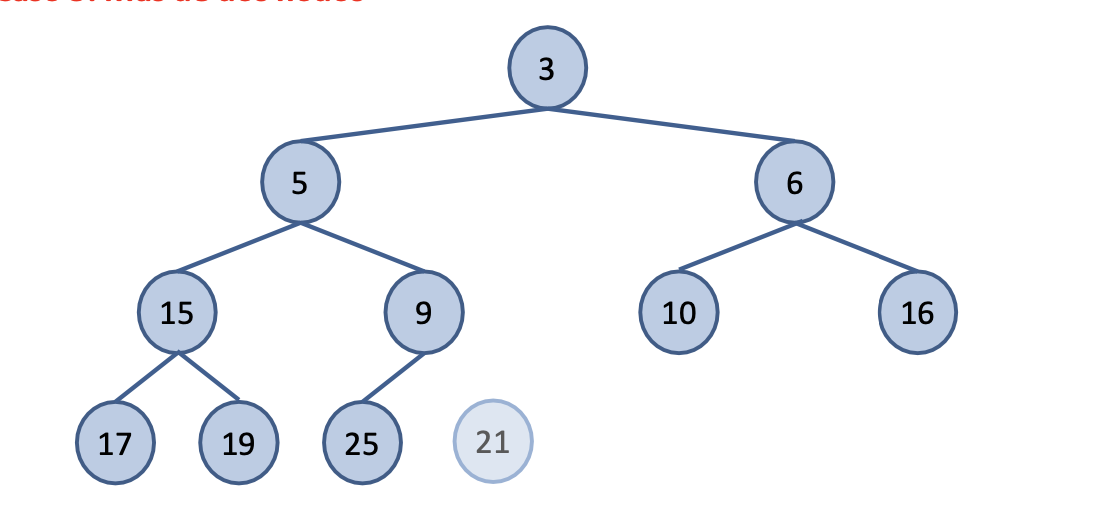
\includegraphics[width=0.7\textwidth]{assets/apo4.png}
  \end{center}
\end{figure}

Vemos que queremos realizar la eliminación del nodo raíz con contenido `3', por tanto, el último nodo del árbol `21', ocupará la posición del nodo raíz sobrescribiendo su contenido y por ende tendremos que hundir dicho nodo para que el APO siga ordenado.
\begin{figure}[h]
  \begin{center}
    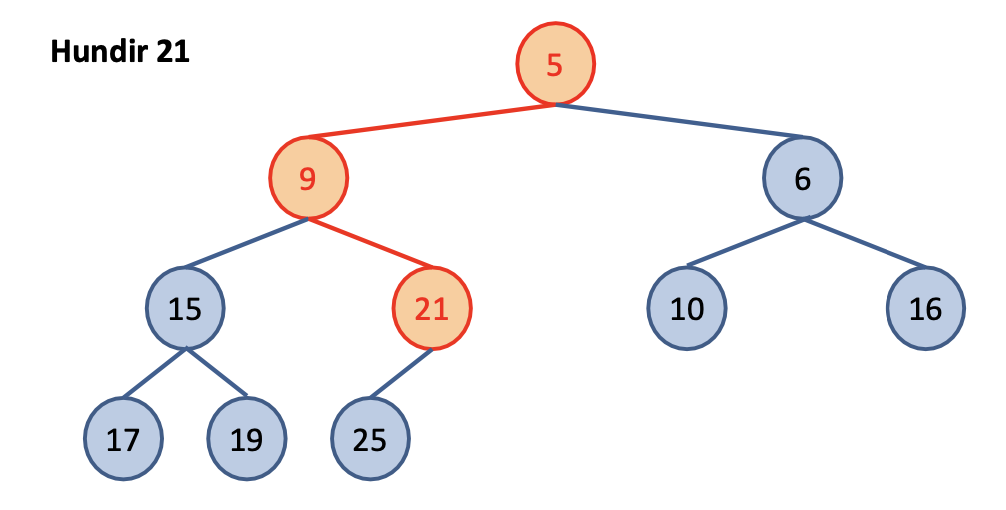
\includegraphics[width=0.7\textwidth]{assets/apo5.png}
  \end{center}
\end{figure}

COmo resultado tenemos que el nodo con valor `21' ahora es padre del nodo con valor `25' y el nuevo nodo raíz es el nodo con valor `5' que previamente era el hijo izquierdo del nodo con valor `3' (la raíz anterior).

\underbar{Código de suprimir:}
\begin{minted}[breaklines]{C++}
template <typename T> void Apo<T>::suprimir(){
  assert(numNodos > 0);
  if(--numNodos > 0){
    nodos[0]=nodos[numNodos];
    if(numNodos > 1)
      hundir(0);
  }
}
\end{minted}
\underbar{Código de hundir:}\\
\begin{minted}[breaklines]{C++}
template <typename T> void Apo<T>::hundir(nodo n){
  bool fin = false;
  T e = nodos[i];
  while (hIzq(i) < numNodos && !fin){
    nodo hMin;
    if (hDer(i) < numNodos && nodos[hDer(i)] 
        < nodos[hIzq(i)])
    hMin = hDer(i);
    else
      hMin = hIzq(i);
      if (nodos[hMin] < e){
        nodos[i] = nodos[hMin];
        i = hMin;
      }
    else
      fin = true;
  }
  nodos[i] = e;
}
\end{minted}
\section{Implementación del TAD APO min y max}
Vamos a realizar la implementación del TAD APO min y máx, donde vamos a poder tener acceso al nodo con valor mínimo y máximo además que vamos a poder eliminar a este último.

Un APO min y max tiene la condición parcial por niveles, los niveles pares tienen una condición diferente a los niveles impares.

En tiempo \((O(1))\) tenemos acceso al mínimo y máximo.

Nivel par → Nodo más pequeño que toda su descendencia.

Nivel impar → Nodo más grande que toda su descendencia.

Para saber si está bien colocado o no:
\begin{enumerate}
  \item Saber en que nivel está ese nodo → Conocemos la posición donde se encuentra almacenado → \(log_2\ h\)  = nivel del árbol.
  \item Dependiendo de si es par o impar el resultado anterior, colocamos el nodo en su sitio para ello flotamos:\\
    1. Comparamos con el padre → si se cumple una vez, se cumple siempre.\\
    2. Comparamos con el abuelo.

\end{enumerate}

Sea el TAD APO min y max:
\begin{minted}[breaklines]{C++}
template <typename T> class APOmM{
  public:
    explicit APOmM(size_t maxNodos); //constructor
    APOmM(const APOmM<T> &A);//ctor de copia
    APOmM<T>& operator=(const APOmM<T> &A);//operador de asignación por copia
    //Modificadores de la clase
    void insertar(const T& e);
    void suprimir();
    void suprimirMax();
    //Observadores de la clase
    const T& cima()const;
    bool vacio()const;
    ~APOmM(); //destructor

  private:
    typedef int nodo; //indice del vector entre 0 y maxNodos-1
    T* nodos; //vector de nodos
    int maxNodos; //Tamaño del vector
    nodo ultimo; //ultimo nodo del APO
    nodo padre(nodo i){return (i==0)? -1 : (i-1)/2;} //Si es la raiz devuelve -1
    nodo hIzq(nodo i){return 2*i+1;}
    nodo hDer(nodo i){return 2*i+2;}
    nodo nodoMinimo(nodo i, nodo j, nodo k);
    nodo nodoMaximo(nodo i, nodo j, nodo k);

    //métodos privados
    void floar(nodo i);
    void hundir(nodo i);
    void Mostrar_descendencia(nodo i);
    void Intercambio(T& a, T& b);

};
//Implementación de los métodos
template <typename T> APOmM<T>::APOmM(size_t maxNodos):nodos(new T[maxNodos]), maxNodos(maxNodos),ultimo(-1){}

template <typename T> ApomM<T>::ApomM(const ApomM<T>& A) : nodos(new T[A.maxNodos]), maxNodos(A.maxNodos),ultimo(A.ultimo){
  // copiar el vector
  for (nodo n = 0; n <= ultimo; n++)
  nodos[n] = A.nodos[n];
}

template <typename T> ApomM<T>& ApomM<T>::operator =(const ApomM<T>& A)
{
  if (this != &A) { // evitar autoasignación
    // Destruir el vector y crear uno nuevo si es necesario
    if (maxNodos != A.maxNodos) {
      delete[] nodos;
      maxNodos = A.maxNodos;
      nodos = new T[maxNodos];
    }
      ultimo = A.ultimo;
      / Copiar el vector
      for (nodo n = 0; n <= ultimo; n++)
      nodos[n] = A.nodos[n];
   }
  return *this;
}
template <typename T> inline const T& ApomM<T>::cima() const{
  assert(ultimo > -1); // ApomM no vacío
  return nodos[0];
}
template <typename T> inline bool ApomM<T>::vacio() const{
  return (ultimo == -1);
}
template <typename T> inline void ApomM<T>::insertar(const T& e){
  //Vamos a insertar por el final del APO
  assert(ultimo < maxNodos-1); // ApomM no lleno
  nodos[++ultimo] = e;
  if (ultimo > 0){
    flotar(ultimo); // Reordenar
  }
}
template <typename T> inline void ApomM<T>::suprimir(){
  assert(ultimo > -1); // ApomM no vacío
  if (--ultimo > -1){ // ApomM no queda vacío
    nodos[0] = nodos[ultimo+1];
    std::cout<<"Va a llamar a hundir"<<std::endl;
  if (ultimo > 0)
    hundir(0); // Quedan dos o más elementos -> Reordenar
  }
}
template <typename T> inline void ApomM<T>::suprimirMax(){
  assert(ultimo > -1);
  if(--ultimo > -1){ //APOmM no queda vacio
    if(ultimo >= 2){ //Tiene 2 hijos y almenos 1 nieto, siendo el máximo uno de los 2 hijos
      if(nodos[1] > nodos[2]){
        nodos[1] = nodos[ultimo+1];
        hundir(1);
      }else{
        nodos[2] = nodos[ultimo+1];
        hundir(2);
      }
    }else if(ultimo == 1){ //Tiene 2 hijos y ningun nieto. Se elimina el hijo derecho y en el izquiero queda el menor
      nodos[1] = std::min(nodos[1],nodos[2]);
    }
  }
}

template <typename T> void ApomM<T>::hundir(nodo i){
  //Ahora hay que determinar profundidad de i, buscar el mayor(nivel impar) o menor(nivel par) nieto y reordenar esos 3
  nodo nietos[4], reordenar[3];
  nodo nietoInter,hijoInter; //El que finalmente se va a intercambiar
  nietos[0] = hIzq(hIzq(i));
  nietos[1] = hDer(hIzq(i));
  nietos[2] = hIzq(hDer(i));
  nietos[3] = hDer(hDer(i));
  std::cout<<"En hundir"<<std::endl;
  int profundidad = log2(i+1);
  if(nietos[0] <=ultimo){
    if(profundidad%2==0){ //Voy a buscar el mínimo de los nietos
      std::cout<<"i está en nivel par"<<std::endl;
      nietoInter = nietos[0];
      if(nietos[1] <= ultimo){
      if(nodos[nietos[1]]<nodos[nietoInter])
        nietoInter=nietos[1];
        if(nietos[2] <=ultimo){
        if(nodos[nietos[2]]<nodos[nietoInter])
          nietoInter=nietos[2];
          if(nietos[3] <=ultimo){
          if(nodos[nietos[3]]<nodos[nietoInter])
            nietoInter=nietos[3];
          }
        }
      }
      hijoInter = padre(nietoInter);
      std::cout<<"Para i= "<<i<<" el nieto a intercambiar es: "<<nietoInter<<" y su padre: "<<hijoInter<<std::endl;
      //Tengo que reordenar a 3 los nodos i, hijoInter, nietoInter
      reordenar[0] = nodoMinimo(i,hijoInter,nietoInter);
      reordenar[1] = nodoMaximo(i,hijoInter,nietoInter);
      if(i != reordenar[0] && i != reordenar[1])
        reordenar[2] = i;
      else if(hijoInter != reordenar[0] && hijoInter != reordenar[1])
        reordenar[2] = hijoInter;
      else if(nietoInter != reordenar[0] && nietoInter != reordenar[1])
        reordenar[2] = nietoInter;
      std::cout<<"El orden al final será: "<<nodos[reordenar[0]]<<"
      "<<nodos[reordenar[1]]<<" "<<nodos[reordenar[2]]<<std::endl;
      T valores[3];
      valores[0] = nodos[reordenar[0]];
      valores[1] = nodos[reordenar[1]];
      valores[2] = nodos[reordenar[2]];
      nodos[i] = valores[0];
      nodos[hijoInter] = valores[1];
      nodos[nietoInter] = valores[2];
      hundir(nietoInter); //Sigo reordenando a partir de nietoInter hacia abajo
    }
    else{ //i está en nivel impar
        std::cout<<"i está en nivel impar"<<std::endl;
        nietoInter = nietos[0];
        if(nietos[1] <= ultimo){
        if(nodos[nietos[1]]>nodos[nietoInter])
          nietoInter=nietos[1];
          if(nietos[2] <=ultimo){
          if(nodos[nietos[2]]>nodos[nietoInter])
            nietoInter=nietos[2];
            if(nietos[3] <=ultimo){
            if(nodos[nietos[3]]>nodos[nietoInter])
              nietoInter=nietos[3];
            }
          }
        }
      std::cout<<"Para i= "<<i<<" el nieto a intercambiar es: "<<nietoInter<<std::endl;
      hijoInter = padre(nietoInter);
      //Tengo que reordenar a 3 los nodos i, hijoInter, nietoInter
      reordenar[0] = nodoMaximo(i,hijoInter,nietoInter);
      reordenar[1] = nodoMinimo(i,hijoInter,nietoInter);
      if(i != reordenar[0] && i != reordenar[1])
        reordenar[2] = i;
      else if(hijoInter != reordenar[0] && hijoInter != reordenar[1])
        reordenar[2] = hijoInter;
      else if(nietoInter != reordenar[0] && nietoInter != reordenar[1])
        reordenar[2] = nietoInter;
      std::cout<<"El orden al final será: "<<nodos[reordenar[0]]<<" "<<nodos[reordenar[1]]<<" "<<nodos[reordenar[2]]<<std::endl;
      T valores[3];
      valores[0] = nodos[reordenar[0]];
      valores[1] = nodos[reordenar[1]];
      valores[2] = nodos[reordenar[2]];
      nodos[i] = valores[0];
      nodos[hijoInter] = valores[1];
      nodos[nietoInter] = valores[2];
      hundir(nietoInter); //Sigo reordenando a partir de nietoInter hacia abajo
    }
    else{
      if(profundidad%2==0){
        nodo hijomin;
        if(hIzq(i) <=ultimo){
          hijomin = hIzq(i);
          if(hDer(i)<=ultimo && nodos[hDer(i)] < nodos[hijomin])
            hijomin = hDer(i);
          if(nodos[hijomin] < nodos[i])
            Intercambio(nodos[hijomin],nodos[i]);
        }
        }
        else{
          nodo hijomax;
          if(hIzq(i) <=ultimo){
            hijomax = hIzq(i);
          if(hDer(i)<=ultimo && nodos[hDer(i)] > nodos[hijomax])
            hijomax = hDer(i);
          if(nodos[hijomax] > nodos[i])
            Intercambio(nodos[hijomax],nodos[i]);
          }
        }
      }
  //Si no hay ni hijos ni nietos, no se hacen llamadas recursivas
  }
}
template <typename T> typename ApomM<T>::nodo ApomM<T>::nodoMinimo(typename ApomM<T>::nodo n1, typename ApomM<T>::nodo n2, typename ApomM<T>::nodo n3){
  if(nodos[n1] < nodos[n2]){
    return (nodos[n1]<nodos[n3]) ? n1 : n3;
  }
  else{ //n2<n1 ( los 3 nodos deberían ser distintos)
    return (nodos[n2]<nodos[n3]) ? n2 : n3;
  }
}
template <typename T> typename ApomM<T>::nodo ApomM<T>::nodoMaximo(typename ApomM<T>::nodo n1, typename ApomM<T>::nodo n2, typename ApomM<T>::nodo n3){
  if(nodos[n1]>nodos[n2]){
    return (nodos[n1]>nodos[n3]) ? n1 : n3;
  }
  else{
    return (nodos[n2]>nodos[n3]) ? n2 : n3;
  }
}
template <typename T> inline ApomM<T>::~ApomM(){
  delete[] nodos;
}
template <typename T> void ApomM<T>::Mostrar_descendencia(ApomM<T>::nodo i){
  //Si i ya no pertenece al arbol o alguno de sus hijos, termina él solito.
  using namespace std;
  if(hIzq(i) <= ultimo){
    cout<<"Hijo izqdo de "<<nodos[i]<<": "<<nodos[hIzq(i)]<<endl;
    Mostrar_descendencia(hIzq(i));
  }
  if(hDer(i) <= ultimo){
    cout<<"Hijo drcho de "<<nodos[i]<<": "<<nodos[hDer(i)]<<endl;
    Mostrar_descendencia(hDer(i));
  }
}


\end{minted}

Finalmente, como conclusión sacamos de que un \textbf{APO} no es un \textbf{AVL}, ya que ambos tienen propositos diferentes, siendo el objetivo principal de los AVLs la búsqueda de elementos lo más rapido posible y en los APOs su uso en algoritmos de ordenación y en el uso de colas con prioridad.
